\documentclass{beamer}
\usepackage{listings}
\usepackage{color}
\usepackage{amsmath}
\usepackage{gvv}

\title{Direction and Normal Vectors}
\author{EE25BTECH11008 - Anirudh M Abhilash}
\date{September 30, 2025}

\begin{document}

%----------------- Title -------------------
\begin{frame}
\titlepage
\end{frame}

%----------------- Problem -------------------
\begin{frame}{Problem Statement}
Find the direction and normal vectors of the line
\[
y = 3x
\]
\end{frame}

%----------------- Solution -------------------
\begin{frame}{Solution}
The equation of the line is
\begin{align}
y &= mx + c \label{eq:genline}
\end{align}

Comparing with $y = 3x$,  
\begin{align}
m &= 3, \quad c = 0
\end{align}

The vector form of the line is
\begin{align}
\vec{x} &= \vec{h} + \kappa \vec{m} \label{eq:vectorform}
\end{align}
\end{frame}

%----------------- Solution (cont) -------------------
\begin{frame}{Solution (cont..)}
Since the line passes through the origin,
\begin{align}
\vec{h} &= \myvec{0 \\ 0}
\end{align}

Thus,
\begin{align}
\vec{x} &= \kappa \myvec{1 \\ 3}
\end{align}

By Comparison, the direction vector is
\begin{align}
\vec{m} &= \myvec{1 \\ m} = \myvec{1 \\ 3}
\end{align}
\end{frame}

\begin{frame}{Solution (cont..)}

For normal vector $\vec{n}$, 
\begin{align}
\vec{n}^\top \vec{m} &= 0
\end{align}

By Solving, the normal vector is
\begin{align}
\vec{n} &= \myvec{-m \\ 1} = \myvec{-3 \\ 1}
\end{align}

\[
\boxed{\vec{m} = \myvec{1 \\ 3}, \quad \vec{n} = \myvec{-3 \\ 1}}
\]
\end{frame}

\begin{frame}[fragile]{Python Code (Plotting Line and Vectors)}
\begin{lstlisting}[language=Python]
import numpy as np
import matplotlib.pyplot as plt

m = 3
c = 0
mvec = np.array([1, m])
nvec = np.array([-1*m, 1])

x_vals = np.linspace(-5, 5, 100)
y_vals = m * x_vals + c

plt.axhline(0, color='black', linewidth=0.5)
plt.axvline(0, color='black', linewidth=0.5)
\end{lstlisting}
\end{frame}

\begin{frame}[fragile]{Python Code (cont..)}
\begin{lstlisting}[language=Python]
plt.plot(x_vals, y_vals, color="green")
plt.text(1+0.2, m*1 + c + 0.2, f"y={m}x+{c}", color="green")

plt.quiver(0, 0, mvec[0], mvec[1], angles='xy', scale_units='xy', scale=1, color='red')
plt.text(mvec[0]*0.6, mvec[1]*0.6, "Direction", color="red")

plt.quiver(0, 0, nvec[0], nvec[1], angles='xy', scale_units='xy', scale=1, color='blue')
plt.text(nvec[0]*0.6, nvec[1]*0.6, "Normal", color="blue")

plt.xlim(-5, 5)
plt.ylim(-5, 5)
plt.grid(True)
plt.gca().set_aspect('equal', adjustable='box')
plt.show()
\end{lstlisting}
\end{frame}

%----------------- Plot -------------------
\begin{frame}[fragile]{Plot}
\begin{figure}[H]\centering
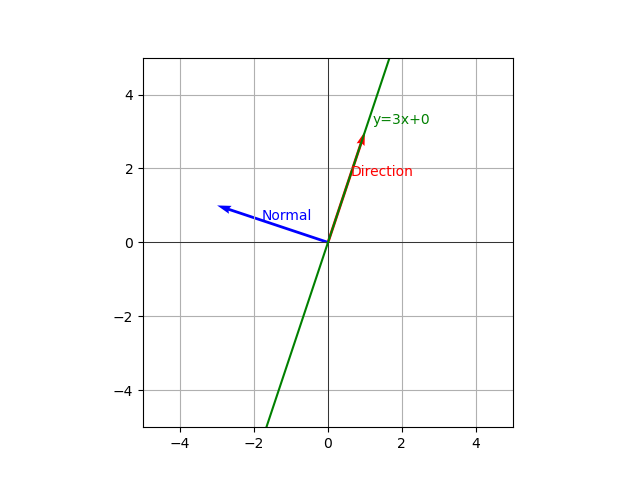
\includegraphics[width=1\columnwidth]{figs/plt.png}
\caption{Parallelogram along with diagonal vectors}
\label{fig:plt}
\end{figure}
\end{frame}

%----------------- C Code -------------------

\begin{frame}[fragile]{C Code (Computations)}
\begin{lstlisting}[language=C]
#include <stdio.h>

void line_vectors(double slope, double* mvec, double* nvec) {
    mvec[0] = 1.0;
    mvec[1] = slope;
    nvec[0] = -slope;
    nvec[1] = 1.0;
}
\end{lstlisting}
\end{frame}


%----------------- Python Code -------------------
\begin{frame}[fragile]{Python Code (Calling C)}
\begin{lstlisting}[language=Python]
import ctypes
import numpy as np
import matplotlib.pyplot as plt

lib = ctypes.CDLL("./vecs.so")

lib.line_vectors.argtypes = [ctypes.c_double,
                             ctypes.POINTER(ctypes.c_double),
                             ctypes.POINTER(ctypes.c_double)]
\end{lstlisting}
\end{frame}

\begin{frame}[fragile]{Python Code (cont..)}
\begin{lstlisting}[language=Python]
def get_vectors(m, c):
    mvec = (ctypes.c_double * 2)()
    nvec = (ctypes.c_double * 2)()
    lib.line_vectors(m, mvec, nvec)
    return np.array([mvec[0], mvec[1]]), np.array([nvec[0], nvec[1]])

m = 3
c = 0

mvec, nvec = get_vectors(m, c)
print("Direction vector m =", mvec)
print("Normal vector n =", nvec)
\end{lstlisting}
\end{frame}

\begin{frame}[fragile]{Python Code (cont..)}
\begin{lstlisting}[language=Python]
x_vals = np.linspace(-5, 5, 100)
y_vals = m * x_vals + c

plt.axhline(0, color='black', linewidth=0.5)
plt.axvline(0, color='black', linewidth=0.5)

plt.plot(x_vals, y_vals, color="green")
plt.text(1+0.2, m*1 + c + 0.2, f"y={m}x+{c}", color="green")
\end{lstlisting}
\end{frame}

\begin{frame}[fragile]{Python Code (cont..)}
\begin{lstlisting}[language=Python]
plt.quiver(0, 0, mvec[0], mvec[1], angles='xy', scale_units='xy', scale=1, color='red')
plt.text(mvec[0]*0.6, mvec[1]*0.6, "Direction", color="red")

plt.quiver(0, 0, nvec[0], nvec[1], angles='xy', scale_units='xy', scale=1, color='blue')
plt.text(nvec[0]*0.6, nvec[1]*0.6, "Normal", color="blue")

plt.xlim(-5, 5)
plt.ylim(-5, 5)
plt.grid(True)
plt.gca().set_aspect('equal', adjustable='box')
plt.show()
\end{lstlisting}
\end{frame}

\end{document}